\chapter{Divisor de potencia Wilkinson}

\section*{Resumen}

En este capítulo se presenta el diseño, simulación, construcción y caracterización de un divisor de potencia Wilkinson de tres puertos, utilizado como parte de la arquitectura de radiofrecuencia del sistema desarrollado.

\section{Introducción}

Los divisores de potencia constituyen elementos fundamentales en el sistema, debido a que permiten distribuir una señal entre diferentes ramas manteniendo determinadas condiciones de adaptación y aislamiento.

En este proyecto se seleccionó una arquitectura basada en un divisor de potencia Wilkinson, debido a que permite obtener una división equitativa de potencia y, simultáneamente, proporcionar adaptación en sus tres puertos y aislamiento entre sus salidas.

El diseño se realizó utilizando líneas de transmisión de un cuarto de longitud de onda implementadas mediante tecnología microstrip. Para una división equitativa, las líneas presentan una impedancia característica de $Z_0\sqrt{2}$, mientras que la resistencia de aislamiento posee un valor de $2Z_0$, considerando una impedancia de referencia $Z_0$.

El objetivo de este capítulo es llevar los fundamentos teóricos del divisor Wilkinson a una implementación física. Para ello, se realiza inicialmente el diseño de las líneas de transmisión, seguido de la simulación del dispositivo, su implementación en PCB y, finalmente, su caracterización experimental.

\section{Especificaciones de diseño}

El diseño del divisor de potencia se realizó considerando como principal condición de operación el intervalo de frecuencias utilizado por el sistema de radiofrecuencia. Las especificaciones adoptadas para el dispositivo se resumen en la Tabla~\ref{tab:especificaciones_wilkinson}.

\begin{table}[H]
\centering
\begin{tabular}{lc}
\hline
\textbf{Parámetro} & \textbf{Especificación} \\
\hline
Tipo de divisor & Wilkinson de 3 puertos \\
División de potencia ideal & $3~\mathrm{dB}$ \\
Número de puertos & 3 \\
Impedancia de referencia & $50~\Omega$ \\
Frecuencia central & $1{,}7~\mathrm{GHz}$ \\
Ancho de banda de interés & $300~\mathrm{MHz}$ \\
Tecnología & Microstrip \\
Sustrato & FR-4 \\
\hline
\end{tabular}
\caption{Especificaciones de diseño del divisor de potencia Wilkinson.}
\label{tab:especificaciones_wilkinson}
\end{table}

Para una división equitativa, cada una de las ramas de salida debe recibir idealmente la mitad de la potencia disponible en el puerto de entrada. Esto es equivalente a una pérdida de inserción ideal de $3~\mathrm{dB}$. Además, se busca obtener una adecuada adaptación en los tres puertos. Estas condiciones constituyen los principales criterios utilizados posteriormente para evaluar el desempeño del dispositivo mediante simulación y medición experimental.

\section{Diseño del divisor Wilkinson}

El diseño del divisor se realizó a partir de la arquitectura teórica presentada en el Capítulo~\ref{chap:wilkinson}. Para una impedancia característica del sistema de $Z_0 = 50~\Omega$, las líneas de transmisión de un cuarto de longitud de onda deben presentar una impedancia característica dada por:

\begin{equation}
    Z_{\lambda/4} = \sqrt{2}Z_0,
\end{equation}

por lo que:

\begin{equation}
    Z_{\lambda/4} = \sqrt{2}(50~\Omega) \approx 70{,}71~\Omega.
\end{equation}

La resistencia de aislamiento ubicada entre los dos puertos de salida debe presentar un valor de:

\begin{equation}
    R = 2Z_0,
\end{equation}

resultando:

\begin{equation}
    R = 100~\Omega.
\end{equation}

Las líneas de transmisión se implementaron utilizando tecnología microstrip. Por lo tanto, la impedancia característica y la longitud eléctrica de las líneas dependen de las propiedades electromagnéticas y geométricas del sustrato utilizado.

Para determinar las dimensiones físicas de las líneas se consideraron la constante dieléctrica relativa del sustrato, su espesor y el espesor del conductor. A partir de estos parámetros se determinó el ancho de pista necesario para obtener una impedancia característica de aproximadamente $70{,}7~\Omega$.

\section{Simulación}

Una vez determinadas las dimensiones iniciales del divisor, se realizó una simulación para evaluar su comportamiento antes de fabricar la placa. El objetivo principal de esta etapa fue verificar la adaptación de los tres puertos, la división de potencia y el aislamiento entre las salidas.

Se utilizó el software \textit{Advanced Design System} (ADS). El asistente de diseño de ADS propone para el divisor Wilkinson una implementación con geometría circular, en la cual las líneas de transmisión de un cuarto de longitud de onda se disponen siguiendo una trayectoria curvada alrededor de un punto central. Esta configuración permite obtener una estructura compacta y mantener la simetría entre las dos ramas de salida. A partir de esta geometría se realizó la simulación y optimización para el sustrato utilizado.

La Figura~\ref{fig:wilkinson_simulacion} presenta el modelo utilizado para la simulación del divisor.

\begin{figure}[H]
    \centering
    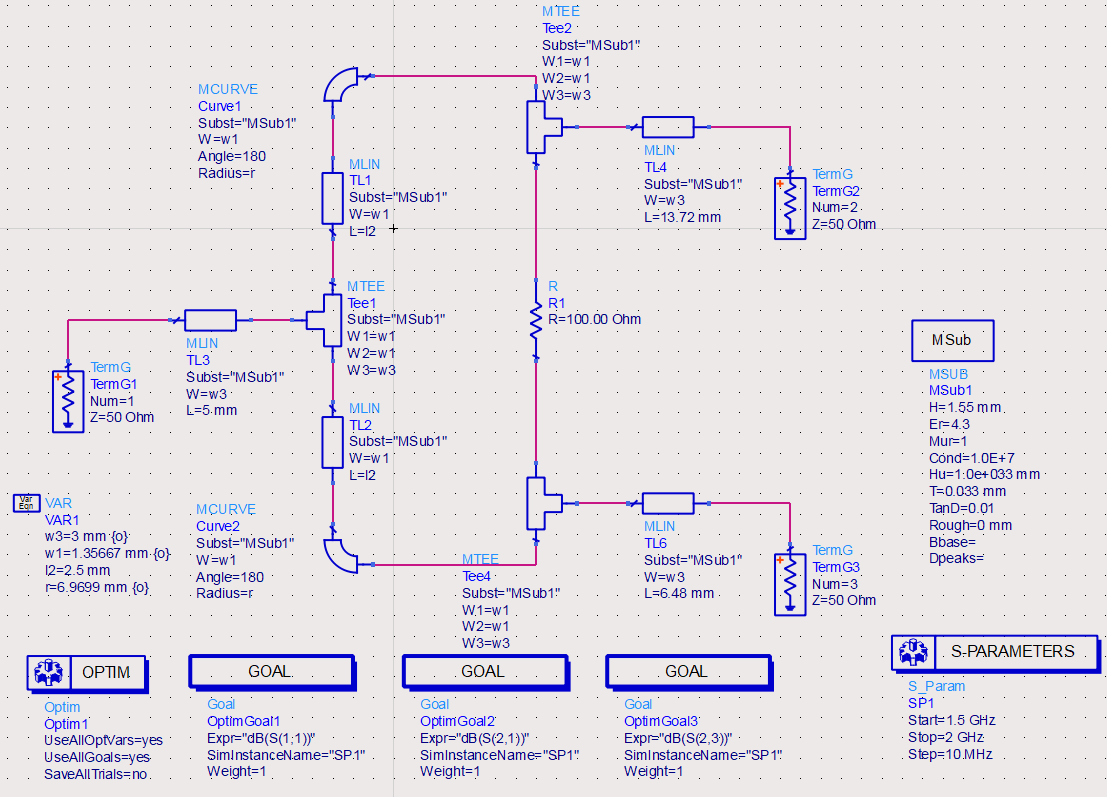
\includegraphics[width=0.85\linewidth]{imagenes/wilkinson_simulacion.png}
    \caption{Modelo del divisor Wilkinson utilizado para la simulación. (Fuente: propia).}
    \label{fig:wilkinson_simulacion}
\end{figure}

Con el objetivo de mejorar el desempeño del divisor de potencia, se realizó una etapa de optimización mediante el motor de optimización de ADS. En esta etapa se definieron como parámetros de interés los coeficientes de dispersión $S_{11}$, $S_{21}$, $S_{31}$ y $S_{23}$, correspondientes a la adaptación del puerto de entrada, la división de potencia hacia cada una de las salidas y el aislamiento entre los puertos de salida, respectivamente. El proceso de optimización permitió ajustar las dimensiones geométricas del divisor. En la Figura~\ref{fig:wilkinson_sparam} se presentan los resultados optimizados del diseño del divisor.

\begin{figure}[H]
    \centering
    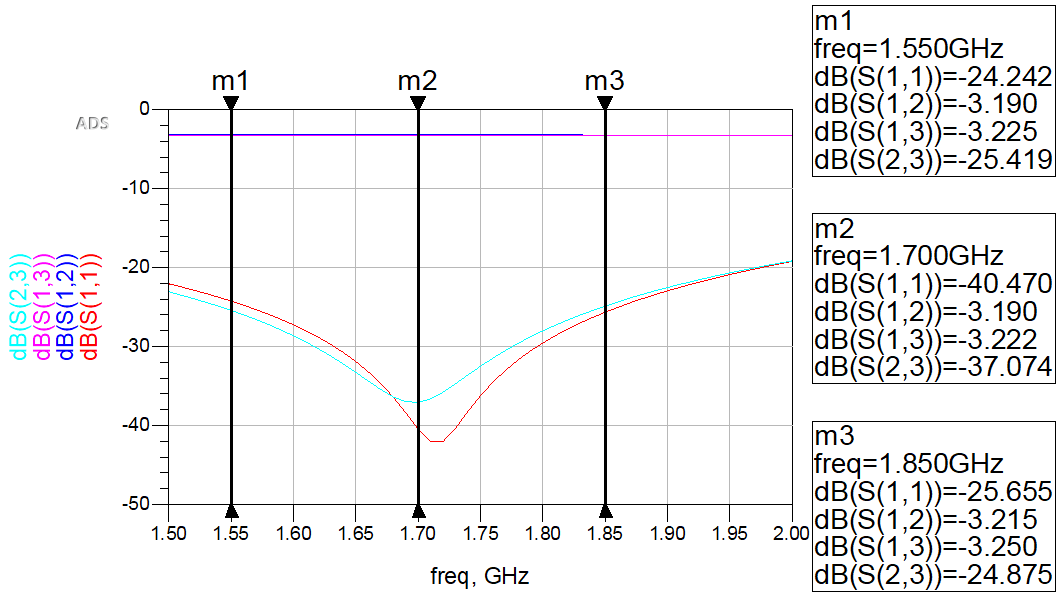
\includegraphics[width=0.85\linewidth]{imagenes/wilkinson_sparam.png}
    \caption{Parámetros de dispersión obtenidos mediante simulación. (Fuente: propia).}
    \label{fig:wilkinson_sparam}
\end{figure}

Una vez finalizado el proceso de optimización, se obtuvo la geometría definitiva del divisor de potencia Wilkinson. En la Figura~\ref{fig:wilkinson_layout} se presenta el \textit{layout} desarrollado en ADS, donde se pueden observar las dos ramas de transmisión de un cuarto de longitud de onda y la resistencia de aislamiento entre los puertos de salida. La geometría mantiene una disposición simétrica respecto del eje central, condición necesaria para obtener una división de potencia equilibrada entre ambas salidas. Este diseño constituye la referencia utilizada posteriormente para la implementación física del divisor en la placa de circuito impreso.

\begin{figure}[H]
    \centering
    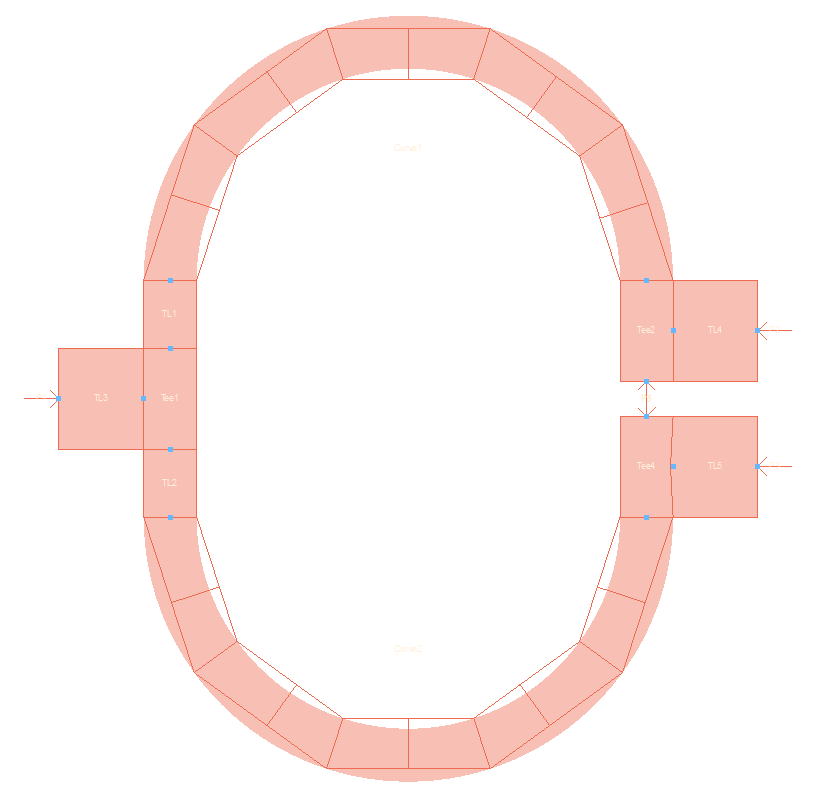
\includegraphics[width=0.5\linewidth]{imagenes/wilkinson_layout.png}
    \caption{Layout final del divisor de potencia Wilkinson obtenido mediante ADS. (Fuente: propia).}
    \label{fig:wilkinson_layout}
\end{figure}

\section{Desarrollo de la placa}

Una vez verificado el comportamiento del diseño mediante simulación, se procedió al desarrollo de la placa de circuito impreso. El diseño se realizó considerando la implementación de las líneas de transmisión mediante tecnología microstrip, manteniendo las dimensiones obtenidas durante la etapa de diseño.

Los componentes utilizados para la construcción del bloque se resumen en la Tabla~\ref{tab:componentes_wilkinson}.

\begin{table}[h]
\centering
\begin{tabular}{lc}
\hline
\textbf{Componente} & \textbf{Característica} \\
\hline
Placa de circuito impreso & FR-4 \\
Resistor & $100~\Omega$ (RT1206DRE07100RL) \\
Conectores & Conector SMA hembra \\
Acabado de PCB & Estaño líquido \\
\hline
\end{tabular}
\caption{Componentes utilizados para la construcción del divisor de potencia Wilkinson.}
\label{tab:componentes_wilkinson}
\end{table}

Posteriormente, la placa fue fabricada y se incorporaron los conectores de RF y la resistencia de aislamiento. La Figura~\ref{fig:wilkinson_pcb} muestra el dispositivo construido.

\begin{figure}[H]
    \centering
    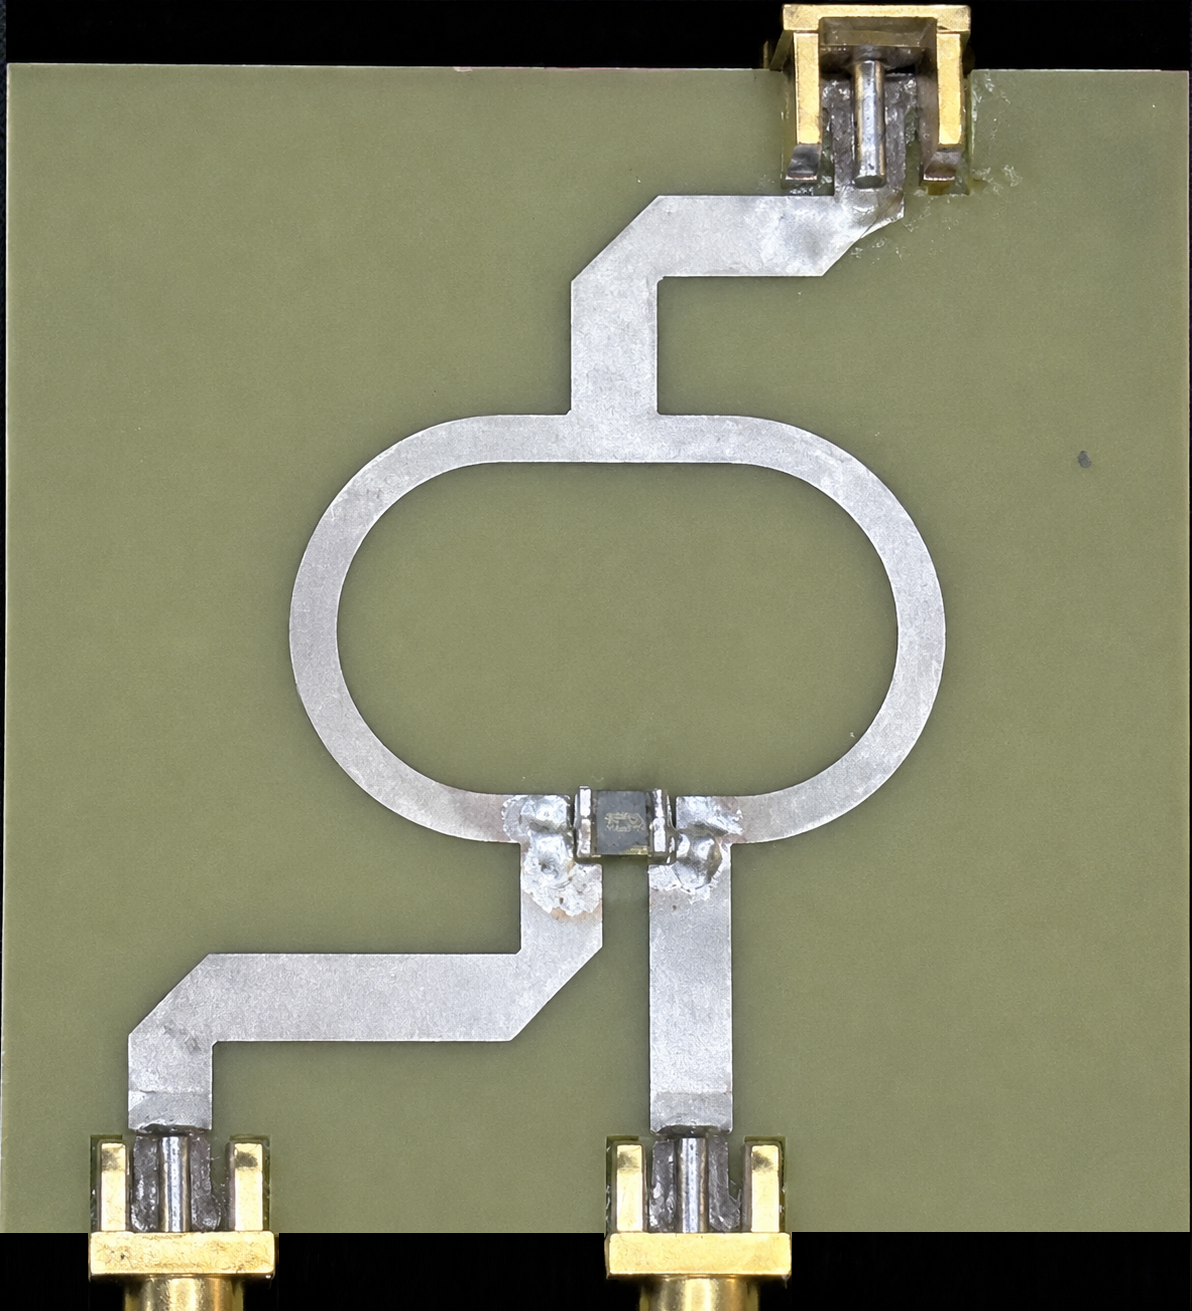
\includegraphics[width=0.3\linewidth]{imagenes/wilkinson_pcb.png}
    \caption{Divisor de potencia Wilkinson construido. (Fuente: propia).}
    \label{fig:wilkinson_pcb}
\end{figure}

A partir del diseño obtenido mediante la simulación, se realizó una modificación de la disposición física del divisor en la placa de circuito impreso. Si bien se mantuvo la geometría definida durante el diseño, la distribución de los elementos y la orientación de los conectores se adaptaron para facilitar la conexión con los módulos que integran el sistema. Esta modificación permite obtener una disposición más conveniente para el montaje y la interconexión del divisor con las etapas posteriores, reduciendo la longitud y complejidad de las conexiones y favoreciendo una implementación más ordenada del conjunto.

\section{Medición del bloque}

Una vez construido el divisor de potencia, se realizó su caracterización experimental mediante un \textit{NanoVNA} previamente calibrado. Posteriormente, se conectó el dispositivo bajo prueba al analizador y se realizaron mediciones en el intervalo de frecuencias de interés, obteniéndose los correspondientes parámetros de dispersión.

En la Figura~\ref{fig:wilkinson_mediciones} se observan las mediciones que permiten evaluar la adaptación de los puertos, analizando las pérdidas de inserción y la impedancia. Por otra parte, los parámetros $S_{21}$ y $S_{31}$ se utilizaron para verificar el equilibrio de potencia entre las dos salidas. Finalmente, el parámetro $S_{23}$ permitió determinar el aislamiento alcanzado entre los puertos de salida.

\begin{figure}[H]
    \centering
    \begin{subfigure}[b]{0.48\linewidth}
        \centering
        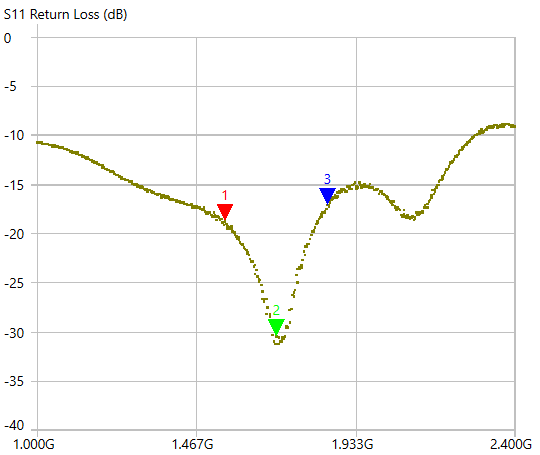
\includegraphics[width=\linewidth]{imagenes/s11_medido.png}
        \caption{$S_{11}$ medido.}
        \label{fig:s11_medido}
    \end{subfigure}
    \hfill
    \begin{subfigure}[b]{0.48\linewidth}
        \centering
        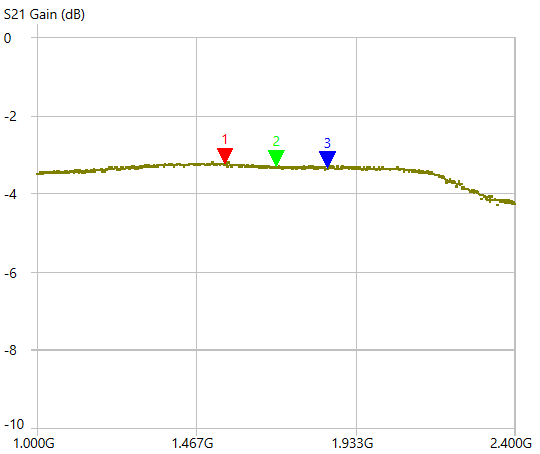
\includegraphics[width=\linewidth]{imagenes/s21_medido.png}
        \caption{$S_{21}$ medido.}
        \label{fig:s21_medido}
    \end{subfigure}

    \vspace{0.5cm}

    \begin{subfigure}[b]{0.48\linewidth}
        \centering
        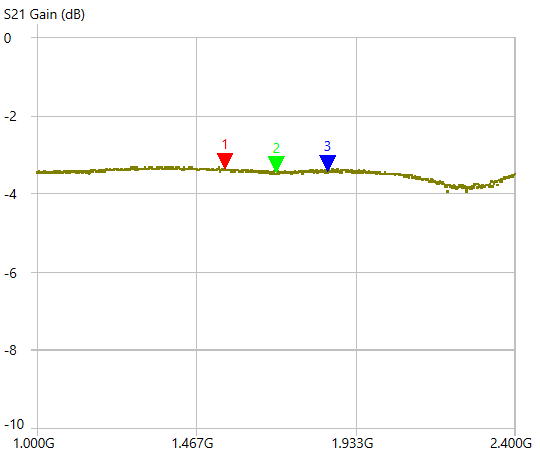
\includegraphics[width=\linewidth]{imagenes/s31_medido.png}
        \caption{$S_{31}$ medido.}
        \label{fig:s31_medido}
    \end{subfigure}
    \hfill
    \begin{subfigure}[b]{0.48\linewidth}
        \centering
        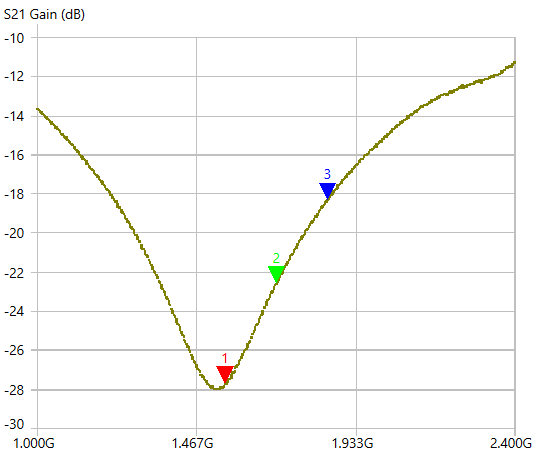
\includegraphics[width=\linewidth]{imagenes/s23_medido.png}
        \caption{$S_{23}$ medido.}
        \label{fig:s23_medido}
    \end{subfigure}

    \caption{Parámetros de dispersión medidos experimentalmente para el divisor de potencia Wilkinson. (Fuente: propia).}
    \label{fig:wilkinson_mediciones}
\end{figure}

A partir de las simulaciones y mediciones realizadas se puede evaluar el cumplimiento de las especificaciones establecidas para el divisor de potencia. La Tabla~\ref{tab:resultados_wilkinson} resume los principales parámetros obtenidos en la frecuencia central.

\begin{table}[H]
\centering
\begin{tabular}{lcc}
\hline
\textbf{Parámetro} & \textbf{Simulado} & \textbf{Medido} \\
\hline
$S_{11}$ & $-40~\mathrm{dB}$ & $-30~\mathrm{dB}$ \\
$S_{21}$ & $-3{,}19~\mathrm{dB}$ & $-3{,}33~\mathrm{dB}$ \\
$S_{31}$ & $-3{,}22~\mathrm{dB}$ & $-3{,}48~\mathrm{dB}$ \\
$S_{23}$ & $-37~\mathrm{dB}$ & $-22{,}6~\mathrm{dB}$ \\
\hline
\end{tabular}
\caption{Comparación entre los resultados simulados y medidos del divisor Wilkinson.}
\label{tab:resultados_wilkinson}
\end{table}
Los resultados muestran un desbalance entre las salidas de $0,15~\mathrm{dB}$. Asimismo, se obtuvo un valor de $S_{11}$ de aproximadamente $-30~\mathrm{dB}$, lo que indica una muy buena adaptación del puerto de entrada. Por otra parte, el aislamiento entre los puertos de salida, representado por $S_{23}$, alcanzó aproximadamente $-22~\mathrm{dB}$, valor que resulta adecuado para la aplicación y evidencia un buen nivel de aislamiento entre ambas salidas.

A partir de las mediciones de impedancia se obtuvieron valores de $49,2+j7,6~\Omega$ para el puerto 2 y de $53+j0,6~\Omega$ para el puerto 3. Estos resultados se encuentran próximos a la impedancia característica de diseño de $50~\Omega$. En particular, el puerto 3 presenta una componente reactiva prácticamente despreciable, mientras que el puerto 2 presenta una componente reactiva ligeramente mayor.